% Options for packages loaded elsewhere
\PassOptionsToPackage{unicode}{hyperref}
\PassOptionsToPackage{hyphens}{url}
%
\documentclass[
  man,floatsintext]{apa6}
\usepackage{amsmath,amssymb}
\usepackage{lmodern}
\usepackage{iftex}
\ifPDFTeX
  \usepackage[T1]{fontenc}
  \usepackage[utf8]{inputenc}
  \usepackage{textcomp} % provide euro and other symbols
\else % if luatex or xetex
  \usepackage{unicode-math}
  \defaultfontfeatures{Scale=MatchLowercase}
  \defaultfontfeatures[\rmfamily]{Ligatures=TeX,Scale=1}
\fi
% Use upquote if available, for straight quotes in verbatim environments
\IfFileExists{upquote.sty}{\usepackage{upquote}}{}
\IfFileExists{microtype.sty}{% use microtype if available
  \usepackage[]{microtype}
  \UseMicrotypeSet[protrusion]{basicmath} % disable protrusion for tt fonts
}{}
\makeatletter
\@ifundefined{KOMAClassName}{% if non-KOMA class
  \IfFileExists{parskip.sty}{%
    \usepackage{parskip}
  }{% else
    \setlength{\parindent}{0pt}
    \setlength{\parskip}{6pt plus 2pt minus 1pt}}
}{% if KOMA class
  \KOMAoptions{parskip=half}}
\makeatother
\usepackage{xcolor}
\IfFileExists{xurl.sty}{\usepackage{xurl}}{} % add URL line breaks if available
\IfFileExists{bookmark.sty}{\usepackage{bookmark}}{\usepackage{hyperref}}
\hypersetup{
  pdftitle={Relations between Inflammation, access to care and Diabetes in two repesentative populations of China and Mexico.},
  pdfauthor={Dominik Grätz1, Rachel Miller-Moudgil1, Amber Somarriba1, Brittany Spinner1, \& Tian Walker1},
  pdflang={en-EN},
  pdfkeywords={Diabetes, access to care, inflammation, health, Mexico, China},
  hidelinks,
  pdfcreator={LaTeX via pandoc}}
\urlstyle{same} % disable monospaced font for URLs
\usepackage{longtable,booktabs,array}
\usepackage{calc} % for calculating minipage widths
% Correct order of tables after \paragraph or \subparagraph
\usepackage{etoolbox}
\makeatletter
\patchcmd\longtable{\par}{\if@noskipsec\mbox{}\fi\par}{}{}
\makeatother
% Allow footnotes in longtable head/foot
\IfFileExists{footnotehyper.sty}{\usepackage{footnotehyper}}{\usepackage{footnote}}
\makesavenoteenv{longtable}
\usepackage{graphicx}
\makeatletter
\def\maxwidth{\ifdim\Gin@nat@width>\linewidth\linewidth\else\Gin@nat@width\fi}
\def\maxheight{\ifdim\Gin@nat@height>\textheight\textheight\else\Gin@nat@height\fi}
\makeatother
% Scale images if necessary, so that they will not overflow the page
% margins by default, and it is still possible to overwrite the defaults
% using explicit options in \includegraphics[width, height, ...]{}
\setkeys{Gin}{width=\maxwidth,height=\maxheight,keepaspectratio}
% Set default figure placement to htbp
\makeatletter
\def\fps@figure{htbp}
\makeatother
\setlength{\emergencystretch}{3em} % prevent overfull lines
\providecommand{\tightlist}{%
  \setlength{\itemsep}{0pt}\setlength{\parskip}{0pt}}
\setcounter{secnumdepth}{-\maxdimen} % remove section numbering
% Make \paragraph and \subparagraph free-standing
\ifx\paragraph\undefined\else
  \let\oldparagraph\paragraph
  \renewcommand{\paragraph}[1]{\oldparagraph{#1}\mbox{}}
\fi
\ifx\subparagraph\undefined\else
  \let\oldsubparagraph\subparagraph
  \renewcommand{\subparagraph}[1]{\oldsubparagraph{#1}\mbox{}}
\fi
\ifLuaTeX
\usepackage[bidi=basic]{babel}
\else
\usepackage[bidi=default]{babel}
\fi
\babelprovide[main,import]{english}
% get rid of language-specific shorthands (see #6817):
\let\LanguageShortHands\languageshorthands
\def\languageshorthands#1{}
% Manuscript styling
\usepackage{upgreek}
\captionsetup{font=singlespacing,justification=justified}

% Table formatting
\usepackage{longtable}
\usepackage{lscape}
% \usepackage[counterclockwise]{rotating}   % Landscape page setup for large tables
\usepackage{multirow}		% Table styling
\usepackage{tabularx}		% Control Column width
\usepackage[flushleft]{threeparttable}	% Allows for three part tables with a specified notes section
\usepackage{threeparttablex}            % Lets threeparttable work with longtable

% Create new environments so endfloat can handle them
% \newenvironment{ltable}
%   {\begin{landscape}\centering\begin{threeparttable}}
%   {\end{threeparttable}\end{landscape}}
\newenvironment{lltable}{\begin{landscape}\centering\begin{ThreePartTable}}{\end{ThreePartTable}\end{landscape}}

% Enables adjusting longtable caption width to table width
% Solution found at http://golatex.de/longtable-mit-caption-so-breit-wie-die-tabelle-t15767.html
\makeatletter
\newcommand\LastLTentrywidth{1em}
\newlength\longtablewidth
\setlength{\longtablewidth}{1in}
\newcommand{\getlongtablewidth}{\begingroup \ifcsname LT@\roman{LT@tables}\endcsname \global\longtablewidth=0pt \renewcommand{\LT@entry}[2]{\global\advance\longtablewidth by ##2\relax\gdef\LastLTentrywidth{##2}}\@nameuse{LT@\roman{LT@tables}} \fi \endgroup}

% \setlength{\parindent}{0.5in}
% \setlength{\parskip}{0pt plus 0pt minus 0pt}

% Overwrite redefinition of paragraph and subparagraph by the default LaTeX template
% See https://github.com/crsh/papaja/issues/292
\makeatletter
\renewcommand{\paragraph}{\@startsection{paragraph}{4}{\parindent}%
  {0\baselineskip \@plus 0.2ex \@minus 0.2ex}%
  {-1em}%
  {\normalfont\normalsize\bfseries\itshape\typesectitle}}

\renewcommand{\subparagraph}[1]{\@startsection{subparagraph}{5}{1em}%
  {0\baselineskip \@plus 0.2ex \@minus 0.2ex}%
  {-\z@\relax}%
  {\normalfont\normalsize\itshape\hspace{\parindent}{#1}\textit{\addperi}}{\relax}}
\makeatother

% \usepackage{etoolbox}
\makeatletter
\patchcmd{\HyOrg@maketitle}
  {\section{\normalfont\normalsize\abstractname}}
  {\section*{\normalfont\normalsize\abstractname}}
  {}{\typeout{Failed to patch abstract.}}
\patchcmd{\HyOrg@maketitle}
  {\section{\protect\normalfont{\@title}}}
  {\section*{\protect\normalfont{\@title}}}
  {}{\typeout{Failed to patch title.}}
\makeatother

\usepackage{xpatch}
\makeatletter
\xapptocmd\appendix
  {\xapptocmd\section
    {\addcontentsline{toc}{section}{\appendixname\ifoneappendix\else~\theappendix\fi\\: #1}}
    {}{\InnerPatchFailed}%
  }
{}{\PatchFailed}
\keywords{Diabetes, access to care, inflammation, health, Mexico, China\newline\indent Word count: X (this cannot easily be done automatically, we can also just leave it out)}
\usepackage{csquotes}
\usepackage[titles]{tocloft}
\cftpagenumbersoff{figure}
\renewcommand{\cftfigpresnum}{\itshape\figurename\enspace}
\renewcommand{\cftfigaftersnum}{.\space}
\setlength{\cftfigindent}{0pt}
\setlength{\cftafterloftitleskip}{0pt}
\settowidth{\cftfignumwidth}{Figure 10.\qquad}
\cftpagenumbersoff{table}
\renewcommand{\cfttabpresnum}{\itshape\tablename\enspace}
\renewcommand{\cfttabaftersnum}{.\space}
\setlength{\cfttabindent}{0pt}
\setlength{\cftafterloftitleskip}{0pt}
\settowidth{\cfttabnumwidth}{Table 10.\qquad}
\ifLuaTeX
  \usepackage{selnolig}  % disable illegal ligatures
\fi

\title{Relations between Inflammation, access to care and Diabetes in two repesentative populations of China and Mexico.}
\author{Dominik Grätz\textsuperscript{1}, Rachel Miller-Moudgil\textsuperscript{1}, Amber Somarriba\textsuperscript{1}, Brittany Spinner\textsuperscript{1}, \& Tian Walker\textsuperscript{1}}
\date{}


\shorttitle{Inflammation, access to care and Diabetes in China and Mexico.}

\authornote{List of group members ordered by alphabet.}

\affiliation{\vspace{0.5cm}\textsuperscript{1} University of Oregon}

\abstract{%
\emph{Background.} Background goes here. \emph{Methods.} Methods go here. \emph{Results.} Results here. \emph{Conclusions.} Conclusions here.
}



\begin{document}
\maketitle

\begin{verbatim}
## 
## Call:
## lm(formula = crp ~ hba1c * medication + age, data = RQ1_df)
## 
## Residuals:
##     Min      1Q  Median      3Q     Max 
## -1.5545 -0.7586 -0.3563  0.5011  3.5249 
## 
## Coefficients:
##                    Estimate Std. Error t value Pr(>|t|)  
## (Intercept)        1.170340   0.621564   1.883   0.0605 .
## hba1c              0.069964   0.039064   1.791   0.0741 .
## medication2        0.859571   0.655572   1.311   0.1906  
## age               -0.002503   0.007024  -0.356   0.7218  
## hba1c:medication2 -0.090588   0.079689  -1.137   0.2564  
## ---
## Signif. codes:  0 '***' 0.001 '**' 0.01 '*' 0.05 '.' 0.1 ' ' 1
## 
## Residual standard error: 1.107 on 366 degrees of freedom
##   (1820 observations deleted due to missingness)
## Multiple R-squared:  0.01194,    Adjusted R-squared:  0.001137 
## F-statistic: 1.105 on 4 and 366 DF,  p-value: 0.3538
\end{verbatim}

\begin{verbatim}
===============================================
                        Dependent variable:    
                    ---------------------------
                                crp            
-----------------------------------------------
hba1c                          0.066           
                              (0.055)          
                                               
dt_exrcse2                     0.010           
                              (0.572)          
                                               
age                           -0.002           
                              (0.007)          
                                               
hba1c:dt_exrcse2              -0.033           
                              (0.069)          
                                               
Constant                      1.335*           
                              (0.686)          
                                               
-----------------------------------------------
Observations                    371            
R2                             0.020           
Adjusted R2                    0.010           
Residual Std. Error      1.103 (df = 366)      
F Statistic             1.901 (df = 4; 366)    
===============================================
Note:               *p<0.1; **p<0.05; ***p<0.01
\end{verbatim}

\begin{verbatim}
## tibble [350 x 10] (S3: tbl_df/tbl/data.frame)
##  $ sex          : Factor w/ 2 levels "1","2": 1 2 1 2 2 1 1 2 1 2 ...
##  $ diagnosis    : Factor w/ 2 levels "1","2": 1 1 1 1 1 1 1 1 1 1 ...
##  $ age          : int [1:350] 67 62 75 87 65 62 60 60 67 57 ...
##  $ hba1c        : num [1:350] 6.54 6.05 14.22 8.82 9.65 ...
##  $ crp          : num [1:350] 0.95 3.15 1.29 1.29 1 ...
##  $ medication   : Factor w/ 2 levels "1","2": 1 1 1 1 1 1 1 1 1 2 ...
##  $ dt_exrcse    : Factor w/ 2 levels "1","2": 2 1 2 1 2 2 2 2 1 2 ...
##  $ med_dt_exrcse: Factor w/ 2 levels "1","2": 2 2 2 2 2 2 2 2 2 1 ...
##  $ access       : Factor w/ 2 levels "1","2": 2 2 2 2 2 1 1 1 1 2 ...
##  $ q5027        : int [1:350] NA NA NA NA NA 1 12 12 1 NA ...
\end{verbatim}

\begin{verbatim}
## tibble [350 x 6] (S3: tbl_df/tbl/data.frame)
##  $ diagnosis: Factor w/ 2 levels "1","2": 1 1 1 1 1 1 1 1 1 1 ...
##  $ age      : int [1:350] 67 62 75 87 65 62 60 60 67 57 ...
##  $ hba1c    : num [1:350] 6.54 6.05 14.22 8.82 9.65 ...
##  $ crp      : num [1:350] 0.95 3.15 1.29 1.29 1 ...
##  $ dt_exrcse: Factor w/ 2 levels "1","2": 2 1 2 1 2 2 2 2 1 2 ...
##  $ access   : Factor w/ 2 levels "1","2": 2 2 2 2 2 1 1 1 1 2 ...
\end{verbatim}

\begin{verbatim}
## 
## Yes  No 
## 158 192
\end{verbatim}

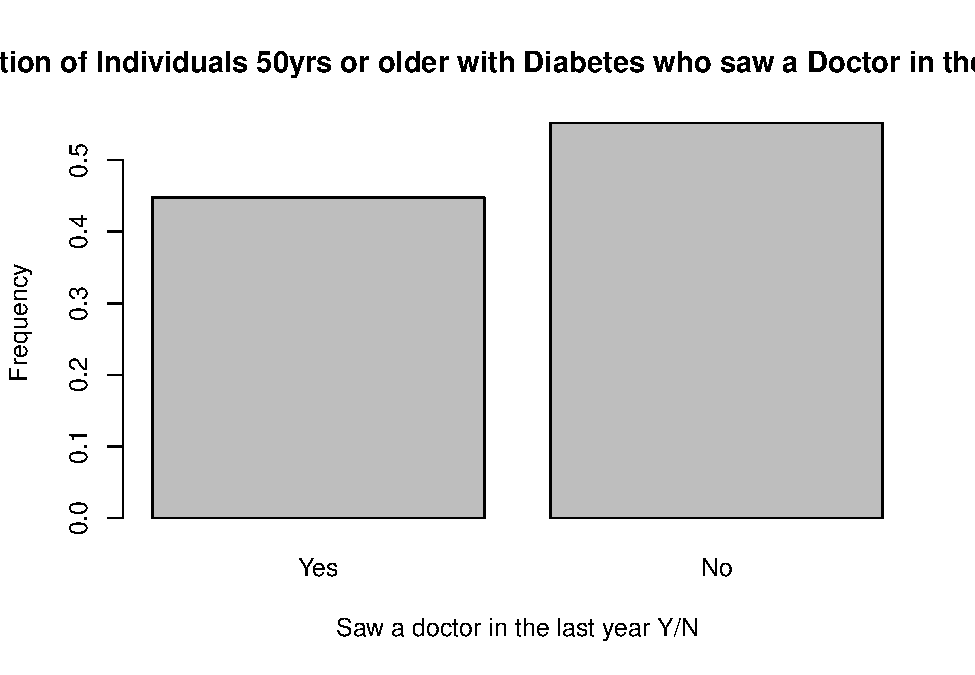
\includegraphics{NEW_Final_Groupof5_files/figure-latex/RQ3-brittany-1.pdf}

\begin{verbatim}
## 
## To cite package 'tidyverse' in publications use:
## 
##   Wickham H, Averick M, Bryan J, Chang W, McGowan LD, François R,
##   Grolemund G, Hayes A, Henry L, Hester J, Kuhn M, Pedersen TL, Miller
##   E, Bache SM, Müller K, Ooms J, Robinson D, Seidel DP, Spinu V,
##   Takahashi K, Vaughan D, Wilke C, Woo K, Yutani H (2019). "Welcome to
##   the tidyverse." _Journal of Open Source Software_, *4*(43), 1686.
##   doi:10.21105/joss.01686 <https://doi.org/10.21105/joss.01686>.
## 
## A BibTeX entry for LaTeX users is
## 
##   @Article{,
##     title = {Welcome to the {tidyverse}},
##     author = {Hadley Wickham and Mara Averick and Jennifer Bryan and Winston Chang and Lucy D'Agostino McGowan and Romain François and Garrett Grolemund and Alex Hayes and Lionel Henry and Jim Hester and Max Kuhn and Thomas Lin Pedersen and Evan Miller and Stephan Milton Bache and Kirill Müller and Jeroen Ooms and David Robinson and Dana Paige Seidel and Vitalie Spinu and Kohske Takahashi and Davis Vaughan and Claus Wilke and Kara Woo and Hiroaki Yutani},
##     year = {2019},
##     journal = {Journal of Open Source Software},
##     volume = {4},
##     number = {43},
##     pages = {1686},
##     doi = {10.21105/joss.01686},
##   }
\end{verbatim}

\begin{verbatim}
## 
## To cite package 'rio' in publications use:
## 
##   Chung-hong Chan, Geoffrey CH Chan, Thomas J. Leeper, and Jason Becker
##   (2021). rio: A Swiss-army knife for data file I/O. R package version
##   0.5.29.
## 
## A BibTeX entry for LaTeX users is
## 
##   @Manual{,
##     title = {rio: A Swiss-army knife for data file I/O},
##     author = {Chung-hong Chan and Geoffrey CH Chan and Thomas J. Leeper and Jason Becker},
##     year = {2021},
##     note = {R package version 0.5.29},
##   }
\end{verbatim}

\begin{verbatim}
## 
## To cite package 'here' in publications use:
## 
##   Müller K (2020). _here: A Simpler Way to Find Your Files_. R package
##   version 1.0.1, <https://CRAN.R-project.org/package=here>.
## 
## A BibTeX entry for LaTeX users is
## 
##   @Manual{,
##     title = {here: A Simpler Way to Find Your Files},
##     author = {Kirill Müller},
##     year = {2020},
##     note = {R package version 1.0.1},
##     url = {https://CRAN.R-project.org/package=here},
##   }
\end{verbatim}

\begin{verbatim}
## 
## To cite package 'papaja' in publications use:
## 
##   Aust, F. & Barth, M. (2022). papaja: Prepare reproducible APA journal
##   articles with R Markdown. R package version 0.1.1. Retrieved from
##   https://github.com/crsh/papaja
## 
## A BibTeX entry for LaTeX users is
## 
##   @Manual{,
##     title = {{papaja}: {Prepare} reproducible {APA} journal articles with {R Markdown}},
##     author = {Frederik Aust and Marius Barth},
##     year = {2022},
##     note = {R package version 0.1.1},
##     url = {https://github.com/crsh/papaja},
##   }
\end{verbatim}

\begin{verbatim}
## 
## To cite package 'tidyr' in publications use:
## 
##   Wickham H, Girlich M (2022). _tidyr: Tidy Messy Data_. R package
##   version 1.2.1, <https://CRAN.R-project.org/package=tidyr>.
## 
## A BibTeX entry for LaTeX users is
## 
##   @Manual{,
##     title = {tidyr: Tidy Messy Data},
##     author = {Hadley Wickham and Maximilian Girlich},
##     year = {2022},
##     note = {R package version 1.2.1},
##     url = {https://CRAN.R-project.org/package=tidyr},
##   }
\end{verbatim}

\begin{verbatim}
## 
## Please cite stargazer in publications as:
## 
##   Hlavac, Marek (2022). stargazer: Well-Formatted Regression and
##   Summary Statistics Tables. R package version 5.2.3.
##   https://CRAN.R-project.org/package=stargazer
## 
## A BibTeX entry for LaTeX users is
## 
##   @Manual{,
##     title = {stargazer: Well-Formatted Regression and Summary Statistics Tables},
##     author = {Marek Hlavac},
##     year = {2022},
##     note = {R package version 5.2.3},
##     organization = {Social Policy Institute},
##     address = {Bratislava, Slovakia},
##     url = {https://CRAN.R-project.org/package=stargazer},
##   }
\end{verbatim}

The descriptive statistics for our sample look as follows:

\begin{longtable}[]{@{}
  >{\raggedright\arraybackslash}p{(\columnwidth - 4\tabcolsep) * \real{0.0541}}
  >{\raggedright\arraybackslash}p{(\columnwidth - 4\tabcolsep) * \real{0.3243}}
  >{\raggedright\arraybackslash}p{(\columnwidth - 4\tabcolsep) * \real{0.6216}}@{}}
\caption{Descriptive statistics.}\tabularnewline
\toprule
\begin{minipage}[b]{\linewidth}\raggedright
\end{minipage} & \begin{minipage}[b]{\linewidth}\raggedright
\end{minipage} & \begin{minipage}[b]{\linewidth}\raggedright
Mexico
\end{minipage} \\
\midrule
\endfirsthead
\toprule
\begin{minipage}[b]{\linewidth}\raggedright
\end{minipage} & \begin{minipage}[b]{\linewidth}\raggedright
\end{minipage} & \begin{minipage}[b]{\linewidth}\raggedright
Mexico
\end{minipage} \\
\midrule
\endhead
\(N_{total}\) & & 2191 \\
Sex & & \\
& male & 869 (39.70 \%) \\
& female & 1317 (60.10 \%) \\
& unknown & 5 (0.20 \%) \\
Age & & 68.20 (\(SD\) = 9.30) \\
Diabetes & & \\
& diagnosed & 374 (17.10 \%) \\
& undiagnosed & 205 (9.40 \%) \\
\bottomrule
\end{longtable}


\clearpage
\renewcommand{\listfigurename}{Figure captions}

\clearpage
\renewcommand{\listtablename}{Table captions}


\end{document}
